% Authored physics chapters. Original source manuscripts remain unchanged.
\part{Quantum models, trained renormalization and physical realizations}
\chapter{Positive evolution, clocks and holonomy}
\label{phys:operators}

A surface order specifies algebraic paths, relations and gluing. A quantum
model additionally specifies a complex Hilbert space, an adjoint, a state,
a Hamiltonian and a measurement rule. Calling a path a clock does not
make those choices. Keeping them explicit turns the physical interpretation
into a sequence of calculable questions.

This part retains finite clocks, infinite observable algebras, quantum field
theory, learned graph networks and molecular hardware. We distinguish a
finite identity, a theorem with hypotheses, a reported experiment and a
proposed design. A conditional arithmetic spectral criterion belongs to the
second category: its missing determinant comparison cannot be supplied by
a hardware analogy.

\section{States and two different logarithms}
A finite system has Hilbert space $\mathcal H=\C^d$, inner product $v^*w$,
and density matrix $\rho=\rho^*\succeq0$, $\operatorname{Tr}\rho=1$.
An observable is Hermitian and has expectation $\operatorname{Tr}(\rho O)$.
A pure state is $vv^*$ for a unit vector $v$; its global phase is invisible.
A self-adjoint energy operator gives two different evolutions:
\begin{equation}\label{phys:evolutions}
 U(t)=e^{-itH/\hbar},\qquad T(a)=e^{-aH/\hbar},\qquad H=H^*.
\end{equation}
Here $t$ and $a$ have time units. The first is unitary, the second positive.
The formal substitution $t=-ia$ is Wick rotation. A continuum field theory
needs additional reconstruction and convergence hypotheses.

\begin{proposition}[Unitary and positive logarithms]\label{phys:logs}
For any unitary $U$ and $\Delta t>0$ there is a bounded self-adjoint $H$
with $U=e^{-iH\Delta t/\hbar}$. For a positive-definite finite matrix $T$,
the matrix $H=-(\hbar/a)\log T$ is Hermitian. These are distinct operations.
\end{proposition}
\begin{proof}
Choose a bounded real Borel argument $\vartheta$ on the circle. Functional
calculus gives $H=-(\hbar/\Delta t)\vartheta(U)$. For the second assertion,
unitary diagonalization of $T$ gives positive eigenvalues $\lambda_j$ and
$\log T=V\operatorname{diag}(\log\lambda_j)V^*$.
\end{proof}
The Borel argument need not be continuous or lie in the original
$C^*$-algebra. The coordinate $z$ on $S^1$ has no continuous logarithm
because of its winding. A singular nilpotent matrix has no matrix logarithm:
every exponential is invertible. One must model such a truncation by a
contraction or channel instead. For a unitary clock, different phase branches
change energies by integer multiples of $2\pi\hbar/\Delta t$; identical
ticks can thus conceal different dynamics between ticks.

For positive $T$, top-eigenvalue normalization has the precise sign
\[
 \widetilde T=T/\lambda_{\max},\qquad
 \widetilde H=H+(\hbar/a)\log\lambda_{\max}\,I\succeq0.
\]
In contrast, $i\log T$ is skew-Hermitian, not this Hamiltonian. If
$\rho>0$ is a density matrix, $K=-\log\rho$ is a dimensionless,
nonnegative modular Hamiltonian. Its interpretation as physical energy
requires a chosen scale and a state-dynamics comparison.

\section{Total positivity, wiring and physical positivity}
A real matrix is totally nonnegative when all minors are nonnegative, and
totally positive when all are positive. These are ordered-basis conditions.
Hilbert-space positivity means Hermitian positive semidefiniteness. The
matrix $\left(\begin{smallmatrix}1&2\\3&7\end{smallmatrix}\right)$ is totally
positive but not Hermitian. Its positive real eigenvalues do not make its
logarithm self-adjoint in the given inner product.

The oscillation theorem and planar-network parametrizations remain valuable
\cite{PhysFominZelevinsky}. In an acyclic directed planar network, the
Lindstr\"om--Gessel--Viennot cancellation expresses a minor of its path
matrix as a sum over disjoint path families. With compatible boundary
orderings the surviving signs are positive. Missing families can give zero
minors, so positive edge weights do not guarantee strict positivity.
Concatenation preserves total nonnegativity, but not symmetry. Positive
Grassmannians organize these minors; they do not alone identify a physical
scattering amplitude or reconstruct a quantum field theory.

\begin{proposition}[A finite positive-energy certificate]
A real symmetric positive-definite transfer matrix has a self-adjoint
logarithmic Hamiltonian. Normalization by its largest eigenvalue makes the
energy nonnegative. Symmetric total positivity is sufficient, not necessary.
\end{proposition}
\begin{proof}
Use Proposition~\ref{phys:logs} and the normalization formula. Only
positivity of the eigenvalues is needed.
\end{proof}

\paragraph{An exactly soluble transfer.}
For $T=\left(\begin{smallmatrix}2&1\\1&2\end{smallmatrix}\right)$, let
$|\pm\rangle=(1,\pm1)^T/\sqrt2$. Its eigenvalues are $3,1$, hence
\[
 T/3=|+\rangle\langle+|+\tfrac13|-\rangle\langle-|,
 \qquad \widetilde H=(\hbar\log3/a)|-\rangle\langle-|.
\]
The normalized state $T/4$ instead has eigenvalues $3/4,1/4$, with modular
energies $\log(4/3),\log4$. Transfer normalization, Gibbs normalization and
energy extraction answer different questions.

For a row-stochastic $P$, detailed balance
$\pi_iP_{ij}=\pi_jP_{ji}$ makes
$S=D^{1/2}PD^{-1/2}$ symmetric, where $D=\operatorname{diag}\pi$.
Its positivity is extra: $P=\left(\begin{smallmatrix}1/4&3/4\\3/4&1/4
\end{smallmatrix}\right)$ is reversible but has eigenvalues $1,-1/2$.
The lazy transition $(I+P)/2$ has eigenvalues $1,1/4$ and a positive
logarithmic interpretation. Laziness changes the process; it is not a
proof of positivity for the original process.

In Euclidean QFT, reflection positivity is a condition on reflected
correlations. Together with the other reconstruction axioms it produces a
Hilbert space and positive-energy translations
\cite{PhysOsterwalderSchrader}. Entrywise nonnegative Boltzmann weights are
not that condition. A family of finite positive matrices does not alone
prove locality, covariance or a continuum limit.

\section{Weyl clocks, Fourier phases and twisted successors}
On $\C^d$ with $\omega=e^{2\pi i/d}$ set
\[
 X_d|j\rangle=|j+1\bmod d\rangle,\qquad
 Z_d|j\rangle=\omega^j|j\rangle.
\]
Acting on basis vectors proves $Z_dX_d=\omega X_dZ_d$ and
$X_d^d=Z_d^d=I$. The unitary Fourier matrix
$(F_d)_{jk}=d^{-1/2}\omega^{jk}$ satisfies $F_dX_dF_d^*=Z_d$.
For a qutrit the explicit matrices are
\[
 X_3=\begin{pmatrix}0&0&1\\1&0&0\\0&1&0\end{pmatrix},\qquad
 Z_3=\operatorname{diag}(1,\omega,\omega^2).
\]
Their commutator $Z_3X_3Z_3^*X_3^*=\omega I$ gives an interference
calibration. The differently ordered product $Z_3X_3X_3^*Z_3^*=I$
contains no Weyl phase. Discrete $X_d,Z_d$ generate a finite Pauli group,
not all of $\mathrm{SU}(d)$. Universality needs suitable continuous
controls and entangling gates.

A successor with wrap-around entry $r\in\C$ obeys
\[
 S_d(r)^d=rI,\qquad
 S_d(r)^*S_d(r)=\operatorname{diag}(1,\ldots,1,|r|^2).
\]
It is unitary precisely when $|r|=1$. For a phase $r=e^{i\phi}$ this is
an explicit twisted clock. A formal uniformizer in a surface order is not
already a complex phase. A representation, specialization and norm must
be supplied before interpreting it physically. A weight with $|r|\le1$
is a contraction, for which ancilla implementation is available below.

\section{Infinite clocks: rotations and odometers are distinct limits}
On $\ell^2(\Z)$ let $U|n\rangle=|n+1\rangle$ and
$V|n\rangle=e^{2\pi i\theta n}|n\rangle$. Then
$VU=e^{2\pi i\theta}UV$. Under Fourier transformation, $U$ becomes
multiplication by $e^{it}$ and $V$ becomes angle translation. They are not
two names for the same multiplication operator. The universal algebra on
this relation is the rotation algebra $A_\theta$.

\begin{proposition}[Finite dimension detects a rational phase]
If $q$-dimensional unitaries satisfy this relation, then $q\theta\in\Z$.
For $\theta=p/q$, the pair $X_q,Z_q^p$ gives a finite representation,
but not a faithful representation of the entire universal $A_{p/q}$.
\end{proposition}
\begin{proof}
Take determinants and cancel the nonzero determinants of $U,V$. At a
rational phase $U^q,V^q$ are central; the finite model fixes them to $I$,
whereas other central circle values are possible.
\end{proof}
The irrational algebra has a canonical trace selecting the coefficient of
$U^0V^0$ in a Fourier polynomial. This is not the ordinary trace of the
identity on an infinite Hilbert space. Abstract algebraic states, normal
states in a representation and trace-class densities are distinct notions.

Continued fractions provide rational approximations
$|\theta-p_j/q_j|<q_j^{-2}$, but the denominators need not divide one
another: successive Fibonacci numbers already refute that assertion.
Exact isometries intertwining both Weyl generators at different phases
would imply $(e^{2\pi i\theta_j}-e^{2\pi i\theta_{j+1}})J=0$, which is
impossible for a nonzero $J$. A limiting construction must specify
approximate embeddings or a continuous field. Elliott--Evans approximations
use matrix algebras over the circle, not a naive AF limit of finite
matrix algebras \cite{PhysElliottEvans}.

A separate infinite clock chooses $n_j\mid n_{j+1}$ and forms
$X=\varprojlim\Z/n_j\Z$. Addition by one is an odometer with Haar
invariant measure. Compatible local extensions
$\C((u^{1/n_j}))/\C((u))$ have these finite cyclic groups. Their inverse
Galois limit and the direct union of fields point in opposite directions.
The full set of denominators gives $\widehat\Z$; a selected tower gives
the corresponding procyclic quotient. This preserves the ramification
interpretation without identifying it with one irrational rotation algebra.

\section{Holonomy, DG compatibility and persistence}
Assign Hilbert fibers to graph vertices and unitary transports to oriented
edges, with inverse on reversed edges. Their based loop product is holonomy;
changing vertex bases conjugates it. For a triangular loop of complex lines
with phases $e^{i\phi_j}$ it is $e^{i(\phi_1+\phi_2+\phi_3)}$.
This is a gauge-invariant phase defect, not yet a gravitational redshift.
\begin{center}
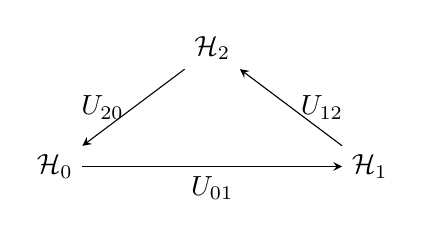
\begin{tikzpicture}[>=stealth]
\node (a) at (0,0) {$\mathcal H_0$};
\node (b) at (4,0) {$\mathcal H_1$};
\node (c) at (2,1.5) {$\mathcal H_2$};
\draw[->] (a)--node[below] {$U_{01}$}(b);
\draw[->] (b)--node[right] {$U_{12}$}(c);
\draw[->] (c)--node[left] {$U_{20}$}(a);
\end{tikzpicture}
\end{center}
Operators on different tensor-product registers instead define many-body
observables. Their product is not automatically transport on one fiber.
The distinction must be fixed before designing a holonomy measurement.

A DG enhancement has $d^2=0$ and a graded Leibniz rule. A clock must
commute with $d$ to act on cohomology. On $\C\xrightarrow{0}\C$, phases
on the two terms can be chosen independently. On
$\C\xrightarrow{1}\C$, compatible scalar actions agree but cohomology
vanishes. Thus the differential alone creates no physical time. Higher
$A_\infty$ operations have their own degrees and signs; periodic syzygies
are not themselves a Hamiltonian or a time period.

A state-derived bifiltration can use increasing spatial radius and a
decreasing correlation threshold. The order must give actual inclusions.
For example, four edges around a square give an $H_1$ class; adding two
triangles fills it. Multiparameter rank invariants, Betti tables and jump
loci are meaningful diagnostics, but there is generally no canonical
complete two-parameter barcode. Stability needs bounds on the actual
filtration functions, including the statistical error of a nonlinear
correlation-to-distance conversion. It does not identify a spectral or
arithmetic determinant.

\chapter{Entanglement and trained quantum renormalization}
\label{phys:learning}

A renormalization channel needs an objective: which observables, states or
phase labels should its coarse variables retain? Training selects parameters
from data. This chapter supplies a solvable optimization task and a graph
extension, while distinguishing an analytic optimum from an executed
training run.

\section{An entangled pair and the finite first law}
Entropy is $S(\rho)=-\operatorname{Tr}(\rho\log\rho)$, with $0\log0=0$.
Reduced states use partial trace; mutual information is
$I(A:B)=S(\rho_A)+S(\rho_B)-S(\rho_{AB})$. We use natural logarithms.
For
\[
 |\psi_p\rangle=\sqrt p|00\rangle+\sqrt{1-p}|11\rangle,\quad0<p<1,
\]
the reductions are $\operatorname{diag}(p,1-p)$, so
$S(\rho_A)=h(p)=-p\log p-(1-p)\log(1-p)$ and $I(A:B)=2h(p)$.
The modular Hamiltonian is
$K_A=\operatorname{diag}(-\log p,-\log(1-p))$. At $p=1/2$ its flow is
trivial although the pair is maximally entangled. Entanglement amount
therefore does not determine a nontrivial local modular clock rate.

\begin{proposition}[Finite first law]
If $\sigma>0$ is a density matrix and $\rho(\epsilon)$ is differentiable,
$\rho(0)=\sigma$, then
\[
 \left.\frac{d}{d\epsilon}S(\rho(\epsilon))\right|_0
 =\operatorname{Tr}(\rho'(0)(-\log\sigma)).
\]
\end{proposition}
\begin{proof}
In a diagonal basis, the derivative under the trace is
$d\operatorname{Tr}(X\log X)[Y]=\operatorname{Tr}(Y(\log X+I))$;
off-diagonal divided-difference terms have zero trace. Use
$\operatorname{Tr}\rho'(0)=0$.
\end{proof}
For the pair above, $h'(p)=\log((1-p)/p)$ is exactly
$\operatorname{Tr}(\operatorname{diag}(1,-1)K_A)$. The reference modular
Hamiltonian stays fixed in this variation. A rank-deficient reference needs
support control or a declared regularization such as
$(1-\eta)\rho+\eta I/d$.

Relative entropy
$D(\rho\Vert\sigma)=\operatorname{Tr}\rho(\log\rho-\log\sigma)$ is
nonnegative, with equality only at equal states; incompatible supports
give infinity. This is a strict matrix-convexity result, not the assertion
that equality in a limit forces equality in an intermediate H\"older
inequality. For the Gibbs state $\sigma=e^{-\beta H}/Z$ one obtains
$K=\beta H+\log Z$. A general reduced state has no automatically identified
physical energy or physical time parameter.

\section{Correlation geometry and the gravitational research question}
On a finite graph assign symmetric regularized lengths
\[
 \ell_e=\ell_*\max\{\varepsilon,
 -\log(\max\{I_e,\delta\}/I_*)\},\qquad
 \ell_*,\varepsilon,\delta,I_*>0.
\]
They define a shortest-path metric. Zero lengths would yield a pseudometric;
infinite lengths could disconnect the graph. If two length assignments
differ by at most $\eta$ on a graph with $N$ vertices, shortest simple
paths have at most $N-1$ edges, hence their distances differ by at most
$(N-1)\eta$. A patchwise bound can be smaller. The logarithm is ill
conditioned near zero correlation, which makes the regularization and its
error propagation part of the model.

A regular tree and $\mathbb H^2$ are both hyperbolic metric spaces but
have different boundaries, Cantor and circle, and are not quasi-isometric.
Negative curvature does not alone give logarithmic diameter for every
finite quotient. Expansion or a controlled family is needed. Arbitrary
edge lengths need not form valid triangles for angle-defect curvature;
metric-only curvature surrogates also require their neighborhood measures.

One can postulate a rate ratio $r_v/r_*=e^{-\alpha\varepsilon_v}$ for
an entanglement proxy. This is a falsifiable ansatz. A bounded cyclic number
expectation cannot increase forever, so an operational rate should use an
unwrapped phase, counted transitions or calibrated oscillations. Matched
noise-only controls must distinguish frequency changes from lost contrast.
The entanglement-equilibrium route to Einstein equations has extra geometric,
area, energy and continuum assumptions \cite{PhysJacobson}. The finite
first law does not supply them. Persistence can test stability across
thresholds; it cannot convert this ansatz into Einstein dynamics.

\section{Pooling is a channel: an exact trainable example}
A channel has Kraus form $\mathcal E(\rho)=\sum_mK_m\rho K_m^*$,
$\sum_mK_m^*K_m=I$. For unitary evolution followed by discarding one qudit,
\[
 \mathcal P_\theta(\rho)=\operatorname{Tr}_2(U_\theta\rho U_\theta^*),
 \qquad K_m=(I\otimes\langle m|)U_\theta.
\]
The completeness identity follows by summing the environment projectors.
An isometry $\C^{d^2}\to\C^d$ would be injective and is impossible for
$d>1$. Stinespring instead adds an environment \cite{PhysStinespring}.
Outcome-dependent unitaries replace $K_m$ by $V_mK_m$. Ignoring the outcome
remains linear; normalization of a selected branch by its success probability
is nonlinear. Partial trace alone is not a nonlinear activation.

\paragraph{A solvable training objective.}
Encode inputs as $R_y(x)|0\rangle\otimes R_y(y)|0\rangle$, where
$R_y(t)=e^{-itY/2}$, and choose
\[
 U_\theta=e^{-i\theta X\otimes X/2},\qquad
 f_\theta(x,y)=\operatorname{Tr}((Z\otimes I)U_\theta\rho_{x,y}U_\theta^*).
\]
This encoding varies with its input; $Z^j|0\rangle$ and
$e^{ix\hat n}|0\rangle$ do not. Anticommutation gives
\[
 U_\theta^*(Z\otimes I)U_\theta
 =\cos\theta(Z\otimes I)+\sin\theta(Y\otimes X),
 \qquad f_\theta(x,y)=\cos\theta\cos x.
\]
The second term averages to zero for these real product states. Before
training, this proves a limitation: that readout cannot retain $y$. Richer
objectives need a changed ansatz or another observable.

For targets $t_j=c\cos x_j$, $-1<c<1$, put
$A=M^{-1}\sum_j\cos^2x_j>0$. The exact squared loss and gradient are
\[
 L(\theta)=A(\cos\theta-c)^2,\qquad
 L'(\theta)=-2A\sin\theta(\cos\theta-c).
\]
The minima satisfy $\cos\theta=c$ and have zero loss. The stationary
points $0,\pi$ must not be mistaken for a trained solution. A numerical
optimizer can be tested against this answer; no run is asserted here.
For comparison, CNOT followed by target-$Z$ readout gives
$f(x,y)=\cos x\cos y$, a true two-input feature.

\begin{center}
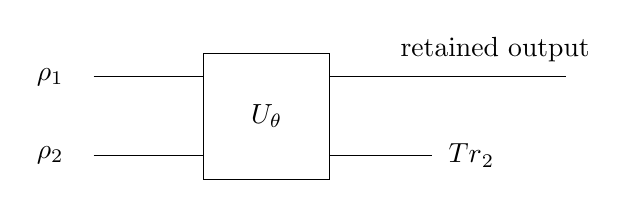
\begin{tikzpicture}[>=stealth]
\draw (0,1)--(6,1);\draw (0,0)--(4.3,0);
\node at (-.55,1) {$\rho_1$};\node at (-.55,0) {$\rho_2$};
\draw[fill=white] (1.4,-.3) rectangle (3,1.3);
\node at (2.2,.5) {$U_\theta$};
\node at (4.8,0) {$\operatorname{Tr}_2$};
\node at (5.1,1.35) {retained output};
\end{tikzpicture}
\end{center}

\section{Trained QGCN and QGAT on ribbon graphs}
Give the graph its cyclic half-edge ordering and a proper edge-coloring.
Shared two-site gates can run in parallel on each color class. A simple
bounded-degree graph requires at most $\Delta+1$ colors, not universally
$\Delta$. Matching-based pooling specifies disjoint retained/discarded
subsystems and a ribbon contraction. Independently applying channels to
overlapping marginals does not automatically produce a consistent global
coarse state.

Quantum convolutional and graph-network proposals offer concrete ansatz
families \cite{PhysCong,PhysZheng,PhysNing}. A trained RG task may target
phase classification, selected correlators, a reconstructed state, or an
effective Hamiltonian. Success on one does not prove success on the others.
A possible loss combines observable errors and symmetry penalties:
\[
 \frac1M\sum_{j,a}w_a(f_{\theta,a}(\rho_j)-t_{j,a})^2
 +\lambda\sum_e|\theta_e-\theta_{\operatorname{rot}(e)}|^2.
\]
The penalty encourages cyclic weight sharing; exact equivariance requires
intertwining by the architecture. Geodesic CNN coordinates and ribbon
orderings are related design inputs, not identical constructions.
Random quanvolutional circuits provide a useful untrained baseline. They
must be compared with trained circuits and a classical model on the same
data rather than credited with an automatic quantum advantage.

For a gate $e^{-i\theta P/2}$ with $P^2=I$, parameter-shift differentiation
gives
\[
 \partial_\theta f=\tfrac12(f(\theta+\pi/2)-f(\theta-\pi/2)).
\]
Indeed the surrounding expectation has only constant, cosine and sine
terms in this parameter. Other generators require a different rule.
Finite-shot gradients and exact-state-vector gradients have different
noise and optimization costs. Clifford layers can create entangled graph
and GHZ states; non-Clifford gates are needed for universality, not for
entanglement itself.

QGAT scores can be obtained from edge-register query/key circuits followed
by classical softmax. For $d>2$, $Z_d$ is not Hermitian, so choose real
quadratures
\[
 C_m=(Z_d^m+Z_d^{-m})/2,\qquad S_m=(Z_d^m-Z_d^{-m})/(2i).
\]
For example,
$s_{vu}=-(\langle C_m\rangle_{q_v}-\langle C_m\rangle_{k_u})^2$ gives
real weights $\alpha_{vu}=e^{\beta s_{vu}}/\sum_we^{\beta s_{vw}}$.
The normalization is classical. The mixture $\sum_u\alpha_{vu}\rho_u$
is a state; a coherent sum of arbitrary unknown value states needs a
separate physical protocol.

Generic amplitude loading of a $D$-component classical vector can cost
order $D$ input operations; $\log D$ qubits do not remove that cost.
Several commuting heads can reuse one measurement basis, but their
expectations still require repeated preparation. Quantum circuits are
linear in $\rho$; nonlinear input encoding and classical processing are
where these feature maps can become nonlinear in classical data.

\section{Associative memory with a correct measurement model}
A normalized readout uses positive effects $E_a$ summing to $I$, with
$p_a=\operatorname{Tr}(E_aU\rho U^*)$. An incomplete readout has sum at
most $I$ and a failure effect. For orthogonal rank-one projectors and pure
input,
\[
 E_a=|\xi_a\rangle\langle\xi_a|,\qquad
 p_a=|\langle U^*\xi_a,\psi\rangle|^2.
\]
This is exact. A common unitary preserves the templates' inner products;
it does not independently prescribe arbitrary nonorthogonal templates.
Arbitrary projectors are not a POVM: two identical $|0\rangle\langle0|$
projectors give probability sum two at $|0\rangle$. A general Hermitian
observable also need not be positive and cannot be interpreted as one
rank-one pattern effect through a generalized square root.

For a two-pattern test, measure the computational basis on $R_y(x)|0\rangle$.
Then $p_0=\cos^2(x/2)$ and $p_1=\sin^2(x/2)$. A larger-probability rule
retrieves zero for $|x|<\pi/2$ modulo $2\pi$. Sampling makes queries near
the boundary difficult. This is a concrete retrieval task, not an
exponential-capacity theorem.

Classical modern Hopfield networks have capacity and retrieval guarantees
under specified separation, normalization and temperature assumptions
\cite{PhysRamsauer}. Substituting $d^{n_q}$ for their associative dimension
does not prove a QGAT memory theorem. A neighborhood with $\delta$ keys
contains $\delta$ explicit candidates per head. Capacity requires a
precision criterion, a dataset and a resource model. A $D$-dimensional
system perfectly distinguishes at most $D$ orthogonal states in one use;
nonorthogonal packing, classical parameter storage and repeated queries
are different resources.

Holographic reduced representations bind classical vectors by circular
convolution. For the unnormalized discrete transform,
$\widehat{a*b}=\widehat a\,\widehat b$. Correlation is an exact inverse
only under additional nonvanishing/normalization conditions. A qudit's
$\langle Z_d^m\rangle=\sum_j\rho_{jj}\omega^{mj}$ determines diagonal
populations when all modes are known, but no off-diagonal phases. Additional
bases distinguish $|+\rangle$ and $|-\rangle$, which have equal populations.

A channel hierarchy can be drawn as a tensor network with coarse bulk
variables and fine boundary variables. Holographic-code models use a
specified isometric encoding and reconstruction property
\cite{PhysPastawski}. Arbitrary discarding does not have it: a channel
sending both $|0\rangle$ and $|1\rangle$ to one state destroys the label.
A pooling tree alone proves neither boundary-area scaling of an actual
state, error-correcting reconstruction nor AdS/CFT. These remain separate
questions that a trained graph model can investigate.

\section{Evidence for trained quantum renormalization}
An executable example must record graph, encoding, task, ansatz, loss,
train/validation split, seed, optimizer and stopping rule. It should save
parameters, predictions and loss history, compare classical and untrained
baselines, and distinguish exact, finite-shot and hardware expectations.
A noise study must name the channel and where it is applied. A successful
finite toy task does not certify a thermodynamic RG limit, quantum speedup,
Einstein dynamics or an arithmetic determinant.

The solvable pooling objective supplies a precise acceptance test for the
separate executable examples. A training result is reported only when
its checkpoint and verification outputs exist. The mathematical model and
its analytic optimum remain meaningful independently of such a run.

\chapter{Noise, molecular spins and hyperbolic-code architectures}
\label{phys:hardware}

An architecture needs controls, interactions, preparation, measurement and
a noise model. A coupling graph supplies none of these calibrations by
itself. Exact small operations provide useful acceptance tests before
considering larger processors or molecular assemblies.

\section{Ancillas, noise and measurement resources}
For a contraction $A$, the map
\[
 v\longmapsto Av\otimes|0\rangle+
       (I-A^*A)^{1/2}v\otimes|1\rangle
\]
is an isometry: its squared norm is $\|v\|^2$. It extends to a unitary
with an environment. Postselecting zero realizes $A$ with probability
$\operatorname{Tr}(A\rho A^*)$. Tracing out the ancilla includes both
branches and does not produce just $A\rho A^*$ as a trace-preserving map.
An operator of norm above one must first be scaled, with its success
probability and amplitude normalization accounted for.

Amplitude damping has Kraus matrices
\[
 K_0=\begin{pmatrix}1&0\\0&\sqrt{1-\gamma}\end{pmatrix},\qquad
 K_1=\begin{pmatrix}0&\sqrt\gamma\\0&0\end{pmatrix},\quad0\le\gamma\le1.
\]
Direct multiplication gives $K_0^*K_0+K_1^*K_1=I$ and multiplies the
excited population by $1-\gamma$. Pure dephasing instead can preserve
populations while reducing coherences. Under a Markovian qubit model,
$1/T_2=1/(2T_1)+1/T_\phi$; these relaxation times alone do not determine
pulse calibration, leakage or gate fidelity.

A Hadamard test estimates $\operatorname{Re}\operatorname{Tr}(\rho U)$;
a changed ancilla basis estimates the imaginary part. Repeated preparations
are required. Local randomized measurements and classical shadows can
reuse settings for many observables, with locality-dependent costs
\cite{PhysShadows}. Entropy is nonlinear, so a linear-observable sample
bound does not automatically estimate mutual information. Reconstructing
small marginals or using dedicated purity/entropy estimators is necessary.

At $N=10^4$ sites and maximum degree $\Delta$, at most $\Delta N/2$
edge marginals are needed. This defines a proposed workload, not an
available processor specification. Routing, state preparation, correlated
readout errors and reset must enter a resource estimate. Likewise $10^5$
qudits of dimension eight require at least $3\times10^5$ binary qubits,
before ancillas and coding. A generic encoded qudit entangler does not
cost merely $\log_2d$ two-qubit gates. Its actual compilation and unused
basis states must be checked. An infinite rotor needs a cutoff and a
bound on leakage/aliasing; a cyclic quotient and a hard truncation have
different boundary behavior.

\section{The peptide-spin evidence and its limits}
Lanthanide-binding peptides offer chemically programmable spin organization.
Rosaleny and collaborators reported ensemble pulsed X-band EPR in frozen
solutions at 4 K, with representative relaxation values
\cite{PhysRosaleny}:
\begin{center}
\begin{tabular}{lcc}
\toprule
Complex & $T_1$ & $T_2$\\\midrule
GdLBT & approximately $10\,\mu$s & approximately $2\,\mu$s\\
NdLBT & approximately $3\,\mu$s & approximately $1\,\mu$s\\\bottomrule
\end{tabular}
\end{center}
Driven nutations motivate a molecular-spin platform, but are not
randomized-benchmark gate fidelities or individual single-shot register
readout. Proposed multispin organization and transport interfaces must
be distinguished from a demonstrated controlled multi-qubit processor.
Binding-affinity improvements are not measurements of increased coherence.

PDB 1TJB is a 2.00 \AA\ Tb-bound structure \cite{PhysNitz}. Its motif has
seventeen amino acids, YIDTNNDGWYEGDELLA, with a terminal amide entry in
the deposited entity. Eight nearby oxygen donors come from Asp3, Asn5,
Asp7, the Trp9 backbone carbonyl, and bidentate Glu11 and Glu14. Deposited
residue identifiers and sequence indices need reconciliation in atomic
constraints. Replacing the metal or scaffold requires new coordination
and magnetic validation; a Tb structural model is not already a calibrated
Gd or Nd control model.

An effective spin Hamiltonian is
\[
 H_{\rm spin}=H_{\rm CF}+\mu_B\mathbf B\cdot\mathbf g\mathbf J
             +\mathbf I\cdot\mathbf A\mathbf J+H_{\rm drive}.
\]
Selecting a qubit requires a named transition, selection rules and leakage
bounds. In a positive-field spin-$7/2$ Zeeman model, the lowest states
have $m=-7/2,-5/2$; the central $-1/2\leftrightarrow1/2$ transition is
not the lowest doublet. Spectroscopic selection can still use it, but
must not be justified by a false energy ordering.

For an ideal two-level splitting $hf$, the thermal polarization is
\[
 p_0-p_1=\tanh\!\left(\frac{hf}{2k_BT}\right).
\]
At $f=9.3$ GHz, $hf/k_B\simeq0.446$ K; at 4 K the polarization is only
about $0.056$. Initialization near a pure state needs a separate protocol.
A peptide's melting temperature and a spin's operational temperature
therefore answer different questions.

\section{Control calculations: rotations and exchange}
Choose the laboratory drive convention
\[
 H(t)=\frac{\hbar\omega_0}{2}Z+
       \hbar\Omega\cos(\omega_0t+\phi)X.
\]
The resonant rotating-wave approximation gives
$H_{\rm rot}=\hbar\Omega(\cos\phi X+\sin\phi Y)/2$ with the stated
rotating-frame convention. For $\phi=0$, a pulse of length $\pi/\Omega$
gives $R_x(\pi)$, equal to $X$ up to phase. A virtual $Z$ changes the
microwave reference phase; avoiding a separate physical pulse does not
mean infinite fidelity of all subsequent gates. Spectral separation and
drive strength control the approximation and leakage.

For dimensionless $\mathbf S=\boldsymbol\sigma/2$, isotropic exchange is
$H_{12}=J\mathbf S_1\cdot\mathbf S_2$, with $J$ in energy units. If $P$
swaps qubits, then $P=(I+XX+YY+ZZ)/2$, so
\begin{equation}\label{phys:exchange}
 e^{-itH_{12}/\hbar}=e^{iJt/(4\hbar)}
 \left[\cos\!\left(\frac{Jt}{2\hbar}\right)I
       -i\sin\!\left(\frac{Jt}{2\hbar}\right)P\right].
\end{equation}
Thus $Jt/\hbar=\pi$ gives SWAP up to phase and $\pi/2$ gives
$\sqrt{\mathrm{SWAP}}$. The latter sends $|01\rangle$ to a Bell-type
superposition proportional to $|01\rangle-i|10\rangle$. It is not iSWAP:
an XY Hamiltonian omits the $ZZ$ term and has different evolution.
Whether a peptide pair realizes any of these models needs measurement;
dipolar anisotropy and $g$-tensor orientation can be essential.

Echo decay, nutations, addressability, gate fidelity and single-shot
measurement are distinct experimental tasks. EPR generally measures an
ensemble signal. CISS and spin-dependent transport are possible future
interfaces, requiring a calibrated relation to a qubit observable.
A discussed SOMO--lanthanide exchange energy is not a measured Ln--Ln
exchange across two nanometres. A fitted law $J_0e^{-\kappa r}$ also needs
consistent units: with $J_0=25$ cm$^{-1}$, $\kappa=1$ \AA$^{-1}$ and
$r=20$ \AA, it predicts about $5.2\times10^{-8}$ cm$^{-1}$, not an
order-one coupling. Geometry and chemistry must determine an actual model.

\section{A proposed molecular-design program}
RFdiffusion3 supports atomically conditioned protein design and structural
benchmarks \cite{PhysRFD3}. Prote\'ina-style backbone generation and
BoltzDesign-style inverse-predictor optimization are complementary candidate
methods. None guarantees a target spin coherence time, interaction graph
or gate. A reproducible calculation pins a release, checkpoint, input
schema, atomic identifiers and constraints; generated structures become
preserved inputs for later evaluation. Current RFD3 documentation uses
structured input specifications and its model-specific design interface,
not an assumed legacy RFdiffusion invocation.

A conservative motif workflow fixes a resolved coordination cage, specifies
metal/donor atoms and the intended state, generates surrounding scaffolds,
assigns sequences with fixed motif positions, and tests structure and
metal-aware energetics before synthesis. Hydrogen-bond conditioning is not
a lanthanide coordination validator. RMSD and prediction confidence are
filters, not physical yields or gate measurements. A small-motif benchmark
does not guarantee a pass rate for a seven-motif, 1000-residue assembly.

ThermoGFN-IF can be formulated as a proposed multi-fidelity optimization
\cite{PhysThermoGFN}. SPURS supplies mutation stability predictions,
BioEmu-v1 protein backbone ensembles, and UMA learned atomistic energies
and forces in evaluated domains \cite{PhysSPURS,PhysBioEmu,PhysUMA}.
Model domains matter: BioEmu-v1 does not explicitly represent metal ions
and their donor-oxygen geometry, so it cannot directly certify an intact
Ln cage. All-atom reconstruction and a separately validated metal-aware
calculation would be extra stages. Atom-count throughput is not a
certificate of spin-vibronic accuracy.

For declared dimensionless scores define
$R(x)=\exp(\sum_jw_js_j(x))$. If positive $\Delta\Delta G$ denotes
destabilization, its stability reward contribution should have a negative
sign. A GFlowNet aims to sample terminal candidates proportionally to this
specified reward. Trajectory balance compares full forward/backward path
probabilities to the terminal reward; subtrajectory balance additionally
uses weighted subpath constraints. A unique construction path restricts
the legal backward policy. These definitions can be implemented and tested
without claiming a synthesized or operating processor.

Increasing melting temperature need not monotonically raise a Debye scale,
suppress a particular spin-phonon channel or improve $T_2$. At a fixed
transition frequency, Bose occupation depends on that frequency and the
temperature, not directly on bulk rigidity. A dephasing power law needs
its spectral density, coupling operator and mechanism, including direct
or Raman processes when relevant. One nanosecond of dynamics does not
alone estimate a converged folded/unfolded partition-function ratio.
Proposed tables mapping $\Delta T_m$ to numerical coherence, gate fidelity
and fault tolerance are therefore hypotheses, not measured outcomes.

\section{Hyperbolic kagome geometry and the assembly problem}
A regular $\{p,q\}$ tiling has $p$ sides per face and $q$ faces at a
vertex. At curvature $-1$, a face has angle $2\pi/q$ and area
$\pi(p-2-2p/q)$. In a closed genus-$g$ quotient,
$pF=2E$, $qV=2E$ and $V-E+F=2-2g$. For $\{7,3\}$,
\begin{equation}\label{phys:counts}
 E=42(g-1),\quad V=28(g-1),\quad F=12(g-1),\quad A_f=\pi/3.
\end{equation}
Then $FA_f=4\pi(g-1)$ as Gauss--Bonnet requires. The orientation-preserving
$(2,3,7)$ triangle group has coarea $\pi/21$; a torsion-free subgroup has
index $84(g-1)$. Its reflection triangle has half this area. The Klein
quartic, with usual model $x^3y+y^3z+z^3x=0$, has genus three and
$(V,E,F)=(56,84,24)$. It is not a construction of every proposed quotient.

For a simple cubic tiling graph, its line graph places a qubit at each
edge and joins pairs that share a vertex. Each qubit has four neighbors;
the line graph has $E$ vertices and $2E$ edges. Quotient degeneracies
such as loops or repeated incidences need separate counting. Equal
hyperbolic edge lengths do not automatically become equal Euclidean
separations or physical couplings in an assembly.

A finite graph can be embedded and routed in three-dimensional space,
but this does not create a complete smooth isometric $\mathbb H^2$ in
$\R^3$. A gyroid has varying intrinsic curvature. Schwarz--Pick concerns
holomorphic metric contraction, not an SE(3) protein-placement algorithm.
A finite assembly needs target Euclidean coordinates, distortion and
steric bounds, mechanical constraints and explicit chemical ownership of
shared sites. Kabsch alignment is a least-squares rigid fit; it does not
remove inconsistent global distances. Two independently generated chunks
cannot both contain one supposedly shared physical peptide without an
actual chemical construction realizing that sharing.

\section{CSS codes from boundary maps}
Let a finite connected closed orientable cellulation have
\[
 C_2(\Sigma;\mathbb F_2)\xrightarrow{\partial_2}
 C_1(\Sigma;\mathbb F_2)\xrightarrow{\partial_1}
 C_0(\Sigma;\mathbb F_2),\qquad\partial_1\partial_2=0.
\]
This is a chain complex, not a short exact sequence. Its first homology
is precisely the code's logical information. Put qubits on edges and set
$H_X=\partial_1$, $H_Z=\partial_2^T$. A binary row $x$ defines an
$X$ product and a row $z$ a $Z$ product. Their commutation sign is
$(-1)^{x\cdot z}$, so the boundary identity proves commutation.
The code is the common $+1$ eigenspace in $(\C^2)^{\otimes E}$, not a
binary kernel intersection regarded as that Hilbert space.

\begin{proposition}[Surface-code dimension and distance]
For this genus-$g$ cellulation,
\[
 k=E-\operatorname{rank}H_X-\operatorname{rank}H_Z=2g.
\]
Distance is the smaller weight of a nontrivial primal homology class and
a nontrivial dual homology class.
\end{proposition}
\begin{proof}
Connectedness gives $\operatorname{rank}\partial_1=V-1$, and the
one-dimensional top homology gives $\operatorname{rank}\partial_2=F-1$.
Thus $k=E-V-F+2=2g$. A commuting $Z$ error is a cycle; multiplication by
$Z$ stabilizers changes it by a boundary. A nontrivial logical $Z$ is
therefore a nonzero homology class. The dual argument treats $X$ errors.
\end{proof}
A noncontractible separating curve can be null homologous. Searching one
geometric systole therefore does not certify a code's distance. In a
$\{7,3\}$ code, vertex $X$ checks have weight three and face $Z$ checks
weight seven; a global swap of $X,Z$ conventions also swaps the logical
descriptions.

At genus thirteen, \eqref{phys:counts} gives 504 data qubits and 26 logical
qubits. If $E=1008$, the genus is 25 and $k=50$. The asymptotic rate is
$1/21$. A $\{5,4\}$ cellulation gives $E=20(g-1)$ and rate $1/10$.
Syndrome ancillas add physical resources. Suitable hyperbolic quotient
families have logarithmic distance at constant rate
\cite{PhysBreuckmannTerhal,PhysDelfosse}; topology alone gives no such
lower bound for every quotient, or distance eight for an unspecified
finite surface. A finite certificate needs its incidence matrices and
primal/dual logical-operator search. Logical qubit count grows linearly,
not exponentially, with the number of physical qubits.

\paragraph{A finite acceptance test.}
An $L\times L$ periodic square cellulation, $L\ge3$, has
$V=F=L^2$, $E=2L^2$. Thus $k=2$ and $d=L$: a straight winding row
or column gives an $L$-edge logical cycle in either lattice, and a lifted
winding cycle must traverse at least $L$ edges. This yields
$[[2L^2,2,L]]$ with weight-four checks. The ranks $L^2-1,L^2-1$ verify
$k$ directly. This is a useful exact decoder test before claiming a
larger unprovided hyperbolic instance.

A storage code is not yet a fault-tolerant computer. Generic exchange
and Zeeman terms do not commute with every stabilizer. An $XX$ interaction
meeting a $Z$ check on exactly one site anticommutes with it, giving a
commutator of order the coupling. Syndrome extraction needs ancillas,
controlled operations, reset and measured error models; three exchange
pulses alone do not prove nondemolition parity measurement. A threshold
is conditional on code family, decoder and noise model. Code-capacity
noise with ideal checks and circuit-level noisy checks are different.
A gate estimate from another model cannot be compared to one threshold
and declared fault tolerance.

\section{The arithmetic comparison is still an additional task}
A physical graph, a complex Belyi dessin and a rational arithmetic model
are different data. A passport need not determine a Galois orbit, and one
finite dessin cannot support a faithful action of the entire absolute
Galois group on its finite sheet set. Frobenius requires descent and good
reduction. Measured couplings do not automatically recover an Euler factor.
The earlier finite-field theta benchmark is a concrete comparison test
with its already specified scope, not a global GRH proof.

There is a useful circuit sanity check. XY exchange annihilates $|00\rangle$,
so its exponential fixes it. A network of these gates, on an all-zero
register preceded only by diagonal $Z$ rotations, has a vacuum overlap
that is just a phase. It cannot generate $L$-function zeros. Also
$e^{-izG}$ for Hermitian $G$ is not generally unitary at complex $z$.
Finite products $\prod_p(1-\chi(p)p^{-s})$ are exponential polynomials
in $s$, not degree-$N$ polynomials; their unramified factor zeros have
$\operatorname{Re}s=0$, not the critical line.

A Hilbert--P\'olya proposal still has to identify its determinant with the
same completed arithmetic function, including gamma and conductor factors.
The transformation $\rho\mapsto1-\overline\rho$ fixes a zero on the
critical line; it does not reverse the ordinate. Conjugate twists matter
for complex characters. Chiral symmetry is extra structure. An unbounded
$\pm$-paired self-adjoint spectrum has no Gibbs trace $e^{-\beta H}$;
$e^{-\beta H^2}$ or $e^{-\beta|H|}$ is a different diagnostic. Similarly
$\sqrt{\Delta-1/4}$ needs a spectral restriction away from negative shifted
modes and a treatment of continuous spectrum.

These chapters give finite calculations, trainable channels and concrete
experiments. They preserve the physical research program while leaving
its arithmetic determinant, purity, convergence and positive-realization
obligations explicit. They establish no complete proof of GRH.
